% Created 2017-03-15 Wed 11:36
% Intended LaTeX compiler: pdflatex
\documentclass[11pt]{article}
\usepackage[utf8]{inputenc}
\usepackage[T1]{fontenc}
\usepackage{graphicx}
\usepackage{grffile}
\usepackage{longtable}
\usepackage{wrapfig}
\usepackage{rotating}
\usepackage[normalem]{ulem}
\usepackage{amsmath}
\usepackage{textcomp}
\usepackage{amssymb}
\usepackage{capt-of}
\usepackage{hyperref}
\author{Zheng Tian}
\date{}
\title{Lecture 6: Linear Regression with One Regressor}
\hypersetup{
 pdfauthor={Zheng Tian},
 pdftitle={Lecture 6: Linear Regression with One Regressor},
 pdfkeywords={},
 pdfsubject={},
 pdfcreator={Emacs 25.1.1 (Org mode 9.0.3)}, 
 pdflang={English}}
\begin{document}

\maketitle
\setcounter{tocdepth}{1}
\tableofcontents



\section*{The Linear Regression Model}
\label{sec:org058974b}

\subsection*{What is regression?}
\label{sec:org55e4367}

\subsubsection*{Definition of \textbf{regress} in Merriam-Webster's dictionary}
\label{sec:org594ac17}

Merriam-Webster gives the following definition of the word "regress":
\begin{enumerate}
\item An act or the privilege of going or coming back
\item Movement backward to a previous and especially worse or more
primitive state or condition
\item The act of reasoning backward
\end{enumerate}

\subsubsection*{The meaning of regression in statistics?}
\label{sec:orge39e018}

\begin{itemize}
\item In statistics, regression analysis focus on the conditional mean of the
dependent variable given the independent variables, which is a
function of the values of independent variables.

\item A very simple functional form of a conditional expectation is a linear
function. That is, we can model the conditional mean as follows,

\begin{equation}
\label{eq:genpopreg}
\mathrm{E}(Y \mid X = x) = f(x) = \beta_{0} + \beta_1 x
\end{equation}

The above equation is a \textbf{simple linear regression function}.
\end{itemize}

\subsection*{Research question:}
\label{sec:orgc1f473a}

\begin{quote}
The research question of this application is: Can reducing class size
increase students' test scores?
\end{quote}

\begin{itemize}
\item How can we answer this question?
\end{itemize}

\subsection*{Randomized controlled experiment}
\label{sec:org1a0b4fe}

\begin{itemize}
\item Randomly choose 42 students and divide them into two classes,
with one having 20 students and another having 22.
\item They are
taught with the same subject and by the same teachers.
\item Randomization ensures that it is the difference in class sizes of
the two classes that is the only factor affecting test scores.
\end{itemize}

\subsection*{Compute conditional means}
\label{sec:org14dd650}

\begin{itemize}
\item After a test for both classes, we then compute the expected values
of test scores, given the different class sizes.
\begin{gather*}
\mathrm{E}(TestScore | ClassSize = 20) \\
\mathrm{E}(TestScore | ClassSize = 22)
\end{gather*}

\item Then the effect of class size on test scores is the difference in
the conditional means, i.e.,
\begin{equation*}
\mathrm{E}(TestScore | ClassSize = 20) - \mathrm{E}(TestScore | ClassSize = 22)
\end{equation*}
\end{itemize}

\subsection*{The population regression function for test scores on class sizes}
\label{sec:orgf59d18d}

\begin{itemize}
\item We use a linear regression function to describe the relationship
between test scores and class sizes.

\item The \textbf{population regression function} or the \textbf{population regression
line}

\begin{equation}
\label{eq:popreg-testscore}
\mathrm{E}(TestScore | ClassSzie) = \beta_0 + \beta_1 ClassSize
\end{equation}
\end{itemize}

\subsection*{The simple linear regression model for test scores on class sizes}
\label{sec:orgc7b4926}

\begin{itemize}
\item We can lump all these factors into a single term, and set up a \textbf{simple linear
regression model} as follows,

\begin{equation}
\label{eq:regmodel-testscore}
TestScore = \beta_0 + \beta_1 ClassSize + OtherFactors
\end{equation}

\item If we assume \(\mathrm{E}(OtherFactors | ClassSize) = 0\), then the
simple linear regression model becomes the population regression line.
\end{itemize}

\subsubsection*{A distinction between the population regression function and the population regression model}
\label{sec:orgb18115d}

\begin{description}
\item[{A population regression function}] \begin{itemize}
\item It's a deterministic relation between class size and the expectation of
test scores.

\item However, we cannot compute the exact value of the test score of a
particular observation.
\end{itemize}

\item[{A population regression model}] \begin{itemize}
\item It's a complete description of a data generating process (DGP).
\item The association between test scores and class size is not
deterministic, depending on the value of other factors.
\end{itemize}
\end{description}

\subsection*{An interpretation of the population regression model}
\label{sec:org2f32d7a}

\begin{itemize}
\item Now we have set up the simple linear regression model,
\begin{equation*}
TestScore = \beta_0 + \beta_1 ClassSize + OtherFactors
\end{equation*}
What is \(\beta_1\) and \(\beta_0\) represent in the model?
\end{itemize}

\subsection*{Interpret \(\beta_1\)}
\label{sec:org70930d3}

\begin{itemize}
\item Denote \(\Delta TestScore\) and \(\Delta ClassSize\) to
be their respective change.

\item \textbf{Holding other factors constant}, we have
\[ \Delta TestScore = \beta_1 \Delta ClassSize  \]
where \(\beta_0\) is removed because it is also a constant.

\item Then, we get

\[ \beta_1 = \frac{\Delta TestScore}{\Delta ClassSize} \]

That is, \(\beta_1\) measures the change in the test score resulting
from a \textbf{one-unit change} in the class size.
\end{itemize}

\subsubsection*{Marginal effect}
\label{sec:org5cdb7e2}

\begin{itemize}
\item When \(TestScore\) and
\(ClassSize\) are two continuous variable, we can write \(\beta_1\) as

\[\beta_1 = \frac{\mathrm{d} TestScore}{\mathrm{d} ClassSize}  \]

\item We often call \(\beta_1\) as the \textbf{marginal effect} of the class
size on the test score.
\end{itemize}

\subsubsection*{Holding other things constant}
\label{sec:org0bf9dae}

\begin{itemize}
\item The phrase of "holding other factors constant" is important. Without
it, we cannot disentangle the effect of class sizes on test scores
from other factors.
\item "Holding other things constant" is often expressed
as the notion of \textbf{ceteris paribus}.
\end{itemize}

\subsection*{Interpret \(\beta_0\)}
\label{sec:orgb3ecc8a}

\begin{itemize}
\item \(\beta_0\) is the intercept in the model.
\item Sometimes it bears real
meanings, but sometimes it merely presents as an intercept.
\item In regression model of test scores on class sizes, \(\beta_0\) is the
test score when the class size and other factors are all zero, which
is obviously nonsensical.
\end{itemize}

\subsection*{The general linear regression model}
\label{sec:org6244ba1}

\begin{itemize}
\item Consider two random variables \(Y\) and \(X\). For both, there are \(n\) observations so that
each observation \(i = 1, 2, 3, \ldots\) is associated with a pair of
values of \((X_i, Y_i)\).

\item Then a \textbf{simple linear regression model} that associates \(Y\) with \(X\) is

\begin{equation}
\label{eq:single-regress}
Y_i = \beta_0 + \beta_1 X_i + u_i, \text{ for } i = 1, \ldots, n
\end{equation}

\item \(Y_i\) is called the dependent variable, the regressand, or the LHS
(left-hand side) variable.
\item \(X_i\) is called the independent variable, the regressor, or the RHS
(right-hand side) variable.
\end{itemize}

\subsubsection*{The general linear regression model (cont'd)}
\label{sec:orgb520e2d}

\begin{itemize}
\item \(\beta_{0}\) is the intercept, or the constant term. It can either have
economic meaning or have merely mathematical sense, which determines
the level of the regression line, i.e., the point of intersection
with the Y axis.
\item \(\beta_{1}\) is the slope of the population regression line. Since
\(\beta_1 = \mathrm{d}Y_i/ \mathrm{d}X_i\), it is the marginal effect
of \(X\) on \(Y\). That is, holding other things constant, one unit
change in \(X\) will make \(Y\) change by \(\beta_1\) units.
\item \(u_i\) is the error term. \(u_i = Y_i - (\beta_0 + \beta_1 X_i)\)
incorporates all the other factors besides \(X\) that determine the
value of \(Y\).
\item \(\beta_{0} + \beta_{1}X_{i}\) represents the population regression
function(or the population regression line).
\end{itemize}

\subsection*{An graphical illustration of a linear regression model}
\label{sec:org27aecdb}

\begin{itemize}
\item The relationship between the data points, the population regression
line, and the errors (other factors) are illustrated in Figure \ref{fig:org42b3132}.
\end{itemize}

\begin{figure}[htbp]
\centering
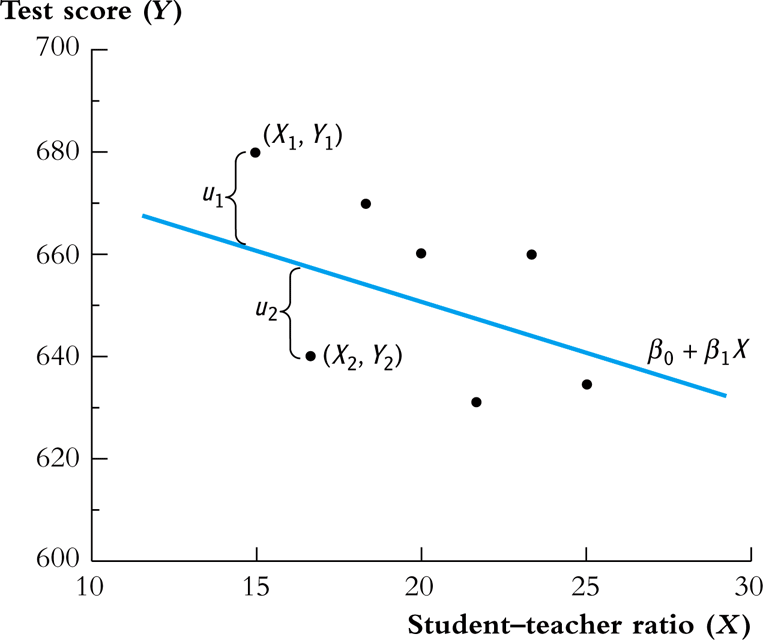
\includegraphics[width=0.75\textwidth]{figure/fig-4-1.png}
\caption{\label{fig:org42b3132}
The Population Regression Line}
\end{figure}


\section*{The OLS Estimation Method for a Linear Regression Model}
\label{sec:orgf6758a4}

\subsection*{The intuition for the OLS and minimization}
\label{sec:orgacf89ca}

\begin{itemize}
\item We use the ordinary least squares (OLS) estimation method to estimate
the simple linear regression model. 
$$Y_i = \beta_0 + \beta_1 X_i + u_i, \text{ for } i = 1, \ldots, n$$
Let's explain the basic idea of the OLS by dissecting its name.
\end{itemize}

\subsubsection*{Ordinary}
\label{sec:org333d6d4}

\begin{itemize}
\item It means that the OLS estimator is a very basic method,
from which we may derive some variations of the OLS
estimator.

\item Other least squares estimators: the weighted least squares (WLS),
and the generalized least squares (GLS).
\end{itemize}

\subsubsection*{Least}
\label{sec:orga472708}

\begin{itemize}
\item It means that the OLS estimator tries to minimize something. The
"something" is the mistakes we make when we try to guess
(estimate) the values of the parameters in the model.

\item If our guess for \(\beta_0\) and \(\beta_1\) is \(b_0\) and \(b_1\), then
the mistake of our guess is 
$$\hat{u}_{i} = Y_{i} - b_0 - b_1 X_i$$
\end{itemize}

\subsubsection*{Squares}
\label{sec:orge85c395}

\begin{itemize}
\item It represent the actual thing (a quantity) that we minimize. The
OLS does not attempt to minimize each \(\hat{u}_{i}\).

\item We minimize the sum of the squared mistakes, 
$$\sum_{i=1}^n \hat{u}_i^2$$
Taking square is to avoid possible offsetting
between positive and negative values of \(\hat{u}_i\) in \(\sum_i
    \hat{u}_i\).
\end{itemize}


\subsection*{The OLS estimators for \(\beta_0\) and \(\beta_1\)}
\label{sec:orge670153}

\begin{itemize}
\item Let \(b_0\) and \(b_1\) be some estimators of \(\beta_0\) and \(\beta_1\),
respectively. Then, the OLS estimators are the solution to the
following minimization problem:
\begin{equation}
\operatorname*{min}_{b_0, b_1}\: S(b_0, b_1) = \sum_{i=1}^n \hat{u}_i^2 = \sum_{i=1}^n (Y_i - b_0 - b_1 X_i)^2 \label{eq:min-ols}
\end{equation}
where \(S(b_0, b_1)\) is a function of \(b_0\) and \(b_1\)
\end{itemize}


\subsection*{The mathematical derivation of the OLS estimators for \(\beta_0\) and \(\beta_1\)}
\label{sec:orgc2c997b}

\subsubsection*{The first order conditions}
\label{sec:org1901fbc}

\begin{itemize}
\item The first order conditions for the minimization problem, evaluated
at the optimal solution \((\hat{\beta}_0, \hat{\beta}_1)\), are

\begin{align}
& \frac{\partial S}{\partial b_0}(\hat{\beta}_0, \hat{\beta}_1) = \sum_{i=1}^n (-2)(Y_i - \hat{\beta}_0 - \hat{\beta}_1 X_i) = 0  \label{eq:b-0} \\
& \frac{\partial S}{\partial b_1}(\hat{\beta}_0, \hat{\beta}_1) = \sum_{i=1}^n (-2)(Y_i - \hat{\beta}_0 - \hat{\beta}_1 X_i) X_i = 0 \label{eq:b-1}
\end{align}
\end{itemize}

\subsubsection*{Get the OLS estimator \(\hat{\beta}_0\)}
\label{sec:org4420fca}

\begin{itemize}
\item From the first condition, we have
\begin{gather}
\sum_{i=1}^n Y_i - n \hat{\beta}_0 - \hat{\beta}_1 \sum_{i=1}^n X_i = 0 \notag  \\
\hat{\beta}_0 = \frac{1}{n} \sum_{i=1}^n Y_i - \frac{\hat{\beta}_1}{n}\sum_{i=1}^n X_i = \overline{Y} - \hat{\beta}_1 \overline{X} \label{eq:bhat-0}
\end{gather}
\end{itemize}

\subsubsection*{Get the OLS estimator \(\hat{\beta}_1\)}
\label{sec:org53349f3}

\begin{itemize}
\item From the second condition, we have
\begin{gather}
\sum_{i=1}^n X_i Y_i - \hat{\beta}_0 \sum_{i=1}^n X_i - \hat{\beta}_1 \sum_{i=1}^n X^2_i = 0  \notag \\
\sum_{i=1}^n X_i Y_i - \frac{1}{n}\sum_{i=1}^n X_i \sum_{i=1}^n Y_i + \hat{\beta}_1 \frac{1}{n} \left(\sum_{i=1}^n X_i\right)^2 - \hat{\beta}_1 \sum_{i=1}^n X_i^2 = 0 \notag \\
\hat{\beta}_1 = \frac{n\sum_{i=1}^n X_i Y_i - \sum_{i=1}^n X_i \sum_{i=1}^n Y_i}{n\sum_{i=1}^n X_i^2 - (\sum_{i=1}^n X_i)^2} \label{eq:bhat-1}
\end{gather}
\end{itemize}

\subsubsection*{A trick of collecting terms}
\label{sec:org6821f0e}

\begin{align*}
\sum_i(X_i - \overline{X})(Y_i - \overline{Y})
&= \sum_i X_iY_i - \overline{X}\sum_iY_i - \overline{Y}\sum_iX_i + \sum_i \overline{X}\overline{Y} \\
&= \sum_i X_iY_i - 2n\overline{X}\overline{Y} + n\overline{X}\overline{Y} \\
&= \sum_i X_iY_i - n\overline{X}\overline{Y} \\
&= \frac{1}{n} \left(n\sum_i X_iY_i - \sum_i X_i \sum_i Y_i\right)
\end{align*}

\begin{itemize}
\item Similarly, we can show that \(\sum_i (X_i - \overline{X})^2 =
  \frac{1}{n} \left[n\sum_i X_i^2 - (\sum_i X_i)^2\right]\).
\end{itemize}

\subsubsection*{Concise expressions of \(\hat{\beta}_1\)}
\label{sec:org49a9049}

\begin{itemize}
\item Collecting terms in the numerator and denominator of
\(\hat{\beta}_1\), we have
\begin{equation*}
\hat{\beta}_1 = \frac{\sum_{i=1}^n (X_i - \overline{X})(Y_i - \overline{Y})}{\sum_{i=1}^n (X_i - \overline{X})^2}
\end{equation*}

\item We can express \(\hat{\beta}_1\) with the sample covariance and the
sample variances of \(X\) and \(Y\).
\begin{itemize}
\item The sample covariance of \(X\) and \(Y\) is \(s_{XY} =
    \frac{1}{n-1} \sum_{i=1}^n (X_i - \overline{X})(Y_i - \overline{Y})\)

\item The sample variance of \(X\) is \(s_X^2 = \frac{1}{n-1} \sum_{i=1}^n
    (X_i - \overline{X})^2\)

\item \(\hat{\beta}_1\) can also be written as
\[ \hat{\beta}_1 = \frac{s_{XY}}{s^2_X}  \]
\end{itemize}
\end{itemize}

\subsubsection*{Summary of the OLS estimators}
\label{sec:org4891322}

\begin{itemize}
\item In sum, solving the minimization problem, we obtain the OLS
estimators for \(\beta_0\) and \(\beta_1\) as

\begin{align}
\hat{\beta}_1 & = \frac{\sum_{i=1}^n (X_i - \overline{X})(Y_i - \overline{Y})}{\sum_{i=1}^n (X_i - \overline{X})^2} = \frac{s_{XY}}{s^2_X}  \label{eq:betahat-1} \\
\hat{\beta}_0 & = \overline{Y} - \hat{\beta}_1 \overline{X}  \label{eq:betahat-0}
\end{align}
\end{itemize}


\subsection*{The predicted values, residuals, and the sample regression line}
\label{sec:org0804e79}

\subsubsection*{The predicted values}
\label{sec:orga8a080f}

\begin{itemize}
\item After obtaining the estimators, we can compute the \textbf{predicted values}
\(\hat{Y}_i\) for \(i=1, \ldots, n\)
$$\hat{Y}_i = \hat{\beta}_0 + \hat{\beta}_1 X_i$$

\item The line represented by the above equation is called \textbf{the sample
regression line}.

\item The sample average point \((\overline{X}, \overline{Y})\) is
always on the sample regression line because
\[ \overline{Y} = \hat{\beta}_0 + \hat{\beta}_1 \overline{X} \]
\end{itemize}

\subsubsection*{The residuals}
\label{sec:org66b66ac}

\begin{itemize}
\item The \textbf{residuals} \(\hat{u}_i\) for \(i = 1, \ldots, n\) are
$$\hat{u}_i = Y_i - \hat{Y}_i$$

\item The residuals are the difference between the observed values of
\(Y_i\) and its predicted value. That is, they are the actual
prediction errors we make when using the OLS estimators.
\end{itemize}


\subsection*{The OLS estimates of the relationship between test scores and the student-teacher ratio}
\label{sec:org1773b75}

\begin{itemize}
\item Now let's come back to the simple linear regression model for test
scores and student-teacher ratios

$$TestScore = \beta_0 + \beta_1 ClassSize + OtherFactors$$

\item Before a formal regression analysis, we often carry out some
preliminary analysis, obtaining some basic statistics and
graphs. Such an analysis is called \textbf{exploratory analysis}
\end{itemize}

\subsubsection*{Basic summary statistics}
\label{sec:org9b0221c}

\begin{itemize}
\item We first need to compute basic summary statistics to see the sample
distribution of the data. Some commonly used summary statistics
include mean, standard deviation, median, minimum, maximum, and
quantile (percentile), etc. 

\begin{table}[htbp]
\caption{\label{tab:org24a7091}
Summary Of distributions of student-teacher ratios and test scores}
\centering
\begin{tabular}{lrrrrrrrrr}
\toprule
 & Average & S.t.d. & 10\% & 25\% & 40\% & 50\% & 60\% & 75\% & 90\%\\
\midrule
\emph{TestScore} & 654.16 & 19.05 & 630.4 & 640.05 & 649.07 & 654.45 & 659.4 & 666.66 & 678.86\\
\emph{STR} & 19.64 & 1.89 & 17.35 & 18.58 & 19.27 & 19.72 & 20.08 & 20.87 & 21.87\\
\bottomrule
\end{tabular}
\end{table}
\end{itemize}

\begin{itemize}
\item Scatterplot
\label{sec:org2be3722}

A scatterplot visualizes the relationship between two variables
straightforwardly, which is helpful for us to decide what a functional
form a regression model should properly take. Figure \ref{fig:orgaf87f21}
shows that test scores and student-teacher ratios may be negatively
related. The correlation coefficient between the two variables is
-0.23, verifying the existence of a weak negative relationship.

\begin{figure}[htbp]
\centering
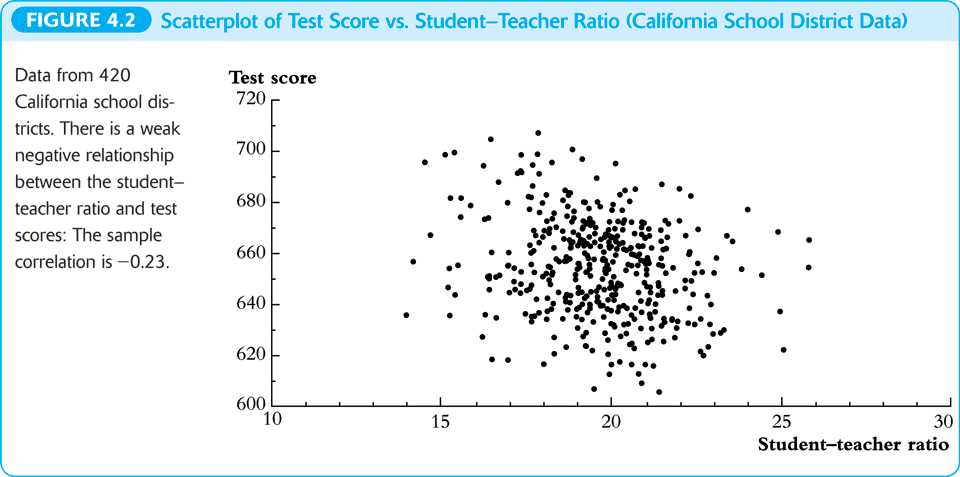
\includegraphics[width=1.0\textwidth]{figure/fig-4-2.png}
\caption{\label{fig:orgaf87f21}
The scatterplot between student-teacher ratios and test scores}
\end{figure}
\end{itemize}

\subsubsection*{Regression analysis}
\label{sec:org9866fbd}

After exploratory analysis, we can estimate the linear model. Although
the formula of computing \(\beta_1\) and \(\beta_0\) (Equations
\ref{eq:betahat-1} and \ref{eq:betahat-0}) seems complicated, the
practical estimation procedure is simplified by using computer
software, like R. For now, let's simply present the estimation
results in the following equation,

\begin{equation}
\label{eq:testscr-str-1e}
\widehat{TestScore} = 698.93 - 2.28 \times STR
\end{equation}

We can draw the sample regression line represented by Equation
\ref{eq:testscr-str-1e} in the scatterplot to eyeball how well the
regression model fits the data.

\begin{figure}[htbp]
\centering
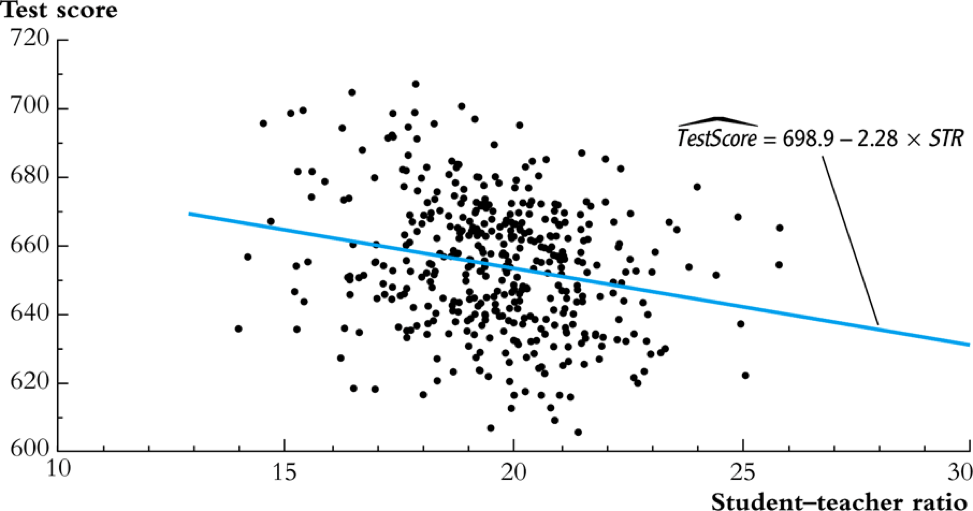
\includegraphics[width=0.85\textwidth]{figure/fig-4-3.png}
\caption{The estimated regression line for the California data}
\end{figure}

\subsubsection*{Interpretation of the estimated coefficients}
\label{sec:orgb58c4de}

Upon obtaining the coefficient estimates, what we need to do next
includes hypothesis tests, model specification tests, robustness (or
sensitivity) test, and interpretation. Let's first see how to
correctly interpret the estimation results.

\begin{itemize}
\item Our main interest is in the slope that tell us how much a unit
change in student-teacher ratios will cause test scores to
change. The slope of -2.28 means that an increase in the
student-teacher ratio by one student per class is, on average,
associated with a decline in district-wide test scores by 2.28
points on the test.
\item The intercept literally means that if the student-teacher ratio is
zero, the average district-wide test scores will be 698.9. However,
it is nonsense for having some positive test scores when the
student-teacher ratio is zero. Therefore, the intercept term in this
case merely serves as determining the level of the sample regression
line.
\item The mere number of -2.28 really does not make much sense for the
readers of your research. We have to put it into the context of
California school district to avoid ridiculous results even though
the estimation itself is correct. (Read the discussion in the
paragraphs in Page 117.)
\end{itemize}
\end{document}